\chapter{Ước lượng mật độ bằng nhân}\label{ch:kde}
\section{Định nghĩa và tính hợp lệ}
Một kernel mật độ thông thường thỏa $K\geq0$, $\int_{\R} K=1$.
Trong các khai triển bậc hai, còn dùng $K$ đối xứng,
$\mu_2(K)=\int u^2K(u)\,du<\infty$ và $R(K)=\int K^2<\infty$.
Với $h>0$,
\[
\boxed{\fhat(x)=\frac1{nh}\sum_{i=1}^n
K\left(\frac{x-X_i}{h}\right).}
\]
Đây là trung bình của $n$ mật độ co giãn, mỗi mật độ có tâm $X_i$.
\begin{proof}[Kiểm tra chuẩn hóa]
Mỗi số hạng không âm, nên $\fhat\geq0$. Trong số hạng thứ $i$,
đặt $u=(x-X_i)/h$, $x=X_i+hu$, $dx=h\,du$:
\[
\int_{\R}\fhat(x)\,dx
=\frac1n\sum_i\int_{\R}\frac1hK((x-X_i)/h)\,dx
=\frac1n\sum_i\int_{\R} K(u)\,du=1.
\]
Tổng hữu hạn cho phép đổi tổng và tích phân. Nhân có phần âm vẫn cho
tích phân 1 nếu khả tích và chuẩn hóa, nhưng không đảm bảo không âm.
\end{proof}

\subsection{KDE liên hệ với EDF như thế nào?}
Đặt $G(t)=\int_{-\infty}^tK(u)\,du$. CDF của KDE là
\[
\widetilde F_{n,h}(x)=\frac1n\sum_iG((x-X_i)/h)
=\int K(u)\Fhat(x-hu)\,du.
\]
Đẳng thức thứ hai đến từ
$\1_{\{X_i\leq x-hu\}}=\1_{\{u\leq(x-X_i)/h\}}$.
Nếu $K$ liên tục, đạo hàm CDF này chính là KDE ở mọi điểm;
với Uniform, đẳng thức đạo hàm đúng hầu khắp nơi.
\intuition{EDF đặt các khối lượng điểm; KDE trải từng khối lượng đó ra
một vùng rộng theo $h$. Tăng $h$ là tăng mức trộn các vùng lân cận.}
\source{\cite{slide2}, slide 19--20; \cite{wasserman}, trang in 132 (PDF 141)}

\section{Bảy kernel và đạo hàm}
Trong bảng dưới, các kernel compact bằng 0 khi $|u|>1$.
Các biểu thức đạo hàm compact được ghi \emph{bên trong} $|u|<1$;
ngoài miền giá đỡ, các đạo hàm bằng 0. Các điểm nối phải kiểm tra riêng.
Đặt $t=|u|$, $\operatorname{sgn}(u)=u/|u|$ khi $u\ne0$.
\begin{longtable}{p{.18\textwidth}p{.74\textwidth}}
\toprule Kernel & $K(u)$, $K'(u)$, $K''(u)$\\\midrule\endhead
Gaussian & $K(u)=\varphi(u)=(2\pi)^{-1/2}e^{-u^2/2}$, $u\in\R$.
\newline $K'(u)=-u\varphi(u)$.
\newline $K''(u)=(u^2-1)\varphi(u)$.\\[5pt]
Epanechnikov & $K(u)=\frac34(1-u^2)$.
\newline $K'(u)=-\frac32u$.
\newline $K''(u)=-\frac32$.\\[5pt]
Uniform & $K(u)=\frac12$.
\newline $K'(u)=0$, $K''(u)=0$.\\[5pt]
Triangular & $K(u)=1-|u|$.
\newline $K'(u)=-\operatorname{sgn}(u)$ nếu $u\ne0$.
\newline $K''(u)=0$ nếu $u\ne0$.\\[5pt]
Biweight & $K(u)=\frac{15}{16}(1-u^2)^2$.
\newline $K'(u)=-\frac{15}{4}u(1-u^2)$.
\newline $K''(u)=\frac{15}{4}(3u^2-1)$.\\[5pt]
Triweight & $K(u)=\frac{35}{32}(1-u^2)^3$.
\newline $K'(u)=-\frac{105}{16}u(1-u^2)^2$.
\newline $K''(u)=-\frac{105}{16}(1-u^2)(1-5u^2)$.\\[5pt]
Tricube & $K(u)=\frac{70}{81}(1-t^3)^3$.
\newline $K'(u)=-\frac{70}{9}ut(1-t^3)^2$.
\newline $K''(u)=-\frac{140}{9}t(1-t^3)(1-4t^3)$.\\
\bottomrule
\end{longtable}
Quy ước $K(\pm1)=1/2$ cho Uniform; các kernel compact còn lại có
$K(\pm1)=0$. Giá trị tại hữu hạn điểm không ảnh hưởng moment nhưng có
thể ảnh hưởng bài tính điểm khi quan sát nằm đúng trên ranh giới.

\subsection{Khả vi tại điểm nối}
\begin{itemize}
\item Gaussian trơn mọi bậc.
\item Uniform không liên tục tại $u=\pm1$, nên không có đạo hàm cổ điển ở đó.
\item Epanechnikov liên tục nhưng không khả vi tại $\pm1$.
\item Triangular không khả vi tại $-1,0,1$.
\item Biweight khả vi liên tục bậc một; $K'(\pm1)=0$, nhưng $K''$
  không tồn tại tại $\pm1$ vì giới hạn độ dốc của $K'$ khác nhau.
\item Triweight khả vi liên tục bậc hai, $K'(\pm1)=K''(\pm1)=0$.
\item Tricube khả vi liên tục bậc hai tại cả $0$ và $\pm1$;
  $K'(0)=K''(0)=K'(\pm1)=K''(\pm1)=0$.
\end{itemize}
Ví dụ, Epanechnikov có đạo hàm từ phía trong tại $u=1$ bằng $-3/2$,
phía ngoài bằng 0. Viết ``$K'(1)=0$ do có chỉ báo'' là sai.
Với Tricube, tính bên $u>0$ rồi dùng tính chẵn của $K$, tính lẻ của
$K'$ để mở rộng; công thức $K''$ là chẵn và liên tục tại 0.

\subsection{Ước lượng đạo hàm mật độ}
Tại một điểm mà mọi số hạng có đạo hàm tương ứng,
\[
\boxed{\widehat f_h'(x)=\frac1{nh^2}\sum_iK'((x-X_i)/h),\qquad
\widehat f_h''(x)=\frac1{nh^3}\sum_iK''((x-X_i)/h).}
\]
Mỗi lần dùng quy tắc dây chuyền, $d[(x-X_i)/h]/dx=1/h$,
nên xuất hiện thêm một thừa số $1/h$.
Nếu một số hạng không khả vi, phải xét \emph{tổng} bằng giới hạn một
phía; các điểm gãy đôi khi có thể triệt tiêu. Không tự kết luận chỉ bằng
tính khả vi của một số hạng.

Đặc biệt, đạo hàm Uniform bằng 0 hầu khắp nơi, nhưng không phải một
ước lượng nhất quán hữu ích của $f'$ thông qua công thức đạo hàm cổ điển.
Đạo hàm theo nghĩa phân phối có khối lượng Dirac ở các bước nhảy;
nó không phải giá trị số của một hàm mật độ đạo hàm thông thường.
Với kernel đủ trơn, phương sai của estimator đạo hàm bậc $q$ có bậc
$1/(nh^{2q+1})$, cho thấy ước lượng đạo hàm khó hơn ước lượng mật độ.
\intuition{Độ trơn của KDE đến từ kernel. ``KDE luôn trơn'' không đúng
với Uniform hoặc Triangular. Muốn tìm độ cong một cách ổn định, nên
dùng kernel có đủ đạo hàm và bandwidth phù hợp với mục tiêu đạo hàm.}

\begin{figure}[htbp]
\centering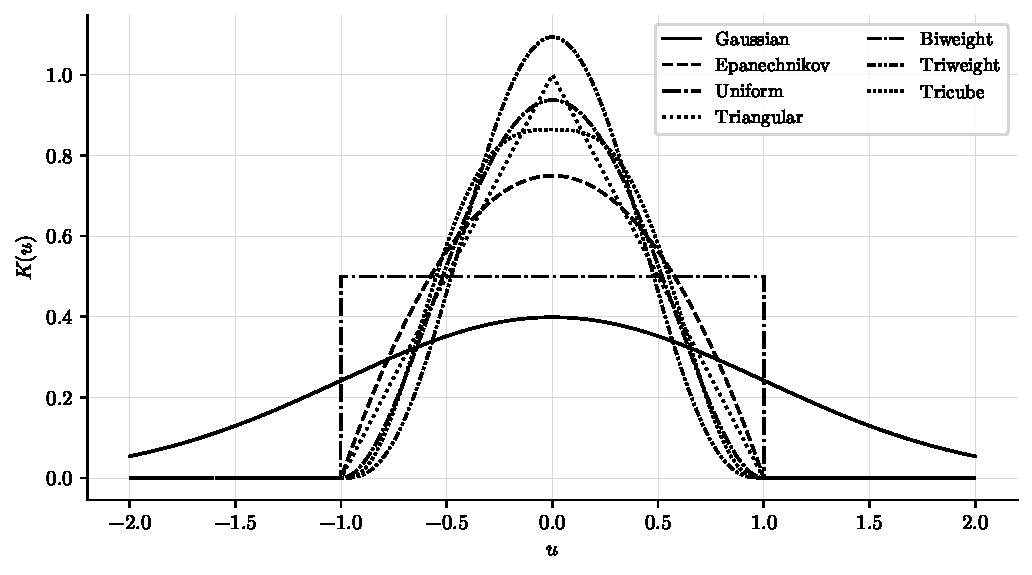
\includegraphics[width=.95\textwidth]{kernels.pdf}
\caption{Bảy kernel đã chuẩn hóa. Tất cả compact có giá đỡ $[-1,1]$;
Gaussian có đuôi trên toàn trục. Hình không thay thế kiểm tra khả vi tại điểm nối.}
\end{figure}

\section{Chứng minh độ chệch của KDE}
Xét điểm nội, hoặc mật độ đủ trơn trên toàn $\R$ mà không có gián đoạn
do biên. Một bộ giả thiết đủ cho khai triển dưới đây là $f\in C^4(\R)$
với đạo hàm bậc bốn bị chặn, $K$ đối xứng,
$\int|u|^4|K(u)|\,du<\infty$, $\int K=1$.
\step{Bước 1: đưa kỳ vọng về tích phân làm trơn.}
Đặt $Z_i(x)=h^{-1}K((x-X_i)/h)$. Tuyến tính cho
$\E\fhat(x)=\E Z_1(x)$. Dùng $u=(x-t)/h$,
\begin{align*}
\E\fhat(x)&=\int\frac1hK((x-t)/h)f(t)\,dt\\
&=\int K(u)f(x-hu)\,du.
\end{align*}
Hệ số $1/h$ triệt tiêu với $h$ trong vi phân; dấu âm của vi phân được
triệt tiêu khi đảo cận.

\step{Bước 2: Taylor đến bậc ba và chặn phần dư.}
\[
f(x-hu)=f(x)-hu f'(x)+\frac{h^2u^2}{2}f''(x)
-\frac{h^3u^3}{6}f'''(x)+\mathcal R_4(x,u,h),
\]
với $|\mathcal R_4|\leq\norm{f^{(4)}}_\infty h^4|u|^4/24$.
Tích phân phần dư nhân $K$ có trị tuyệt đối $O(h^4)$ nhờ moment
tuyệt đối bậc bốn hữu hạn.

\step{Bước 3: dùng moment của kernel.}
Vì kernel chẵn, $uK(u)$ và $u^3K(u)$ lẻ và khả tích, nên tích phân
trên miền đối xứng bằng 0. Vì $\int K=1$,
\begin{align*}
\E\fhat(x)&=f(x)+\frac{h^2}{2}\mu_2(K)f''(x)+O(h^4),\\
\boxed{\Bias(\fhat(x))}&\boxed{=\frac{h^2}{2}\mu_2(K)f''(x)+O(h^4).}
\end{align*}
Nếu chỉ có $f''$ liên tục và điều kiện chi phối phù hợp, kết quả thường
là $h^2\mu_2f''/2+o(h^2)$; không tự nâng phần dư lên $O(h^4)$.

\subsection{Ý nghĩa hình học của độ cong}
Với kernel không âm, $\mu_2(K)>0$. Ở đỉnh cong xuống,
$f''(x)<0$: chệch dẫn đầu âm, KDE trung bình làm thấp đỉnh
(undershoot). Ở đáy cong lên, $f''(x)>0$: chệch dẫn đầu dương,
KDE làm đầy đáy (overshoot). Nếu $f''(x)=0$, số hạng dẫn đầu mất;
cần xem bậc cao hơn thay vì dùng công thức tối ưu chia cho $f''(x)^2$.
\intuition{Làm trơn là lấy trung bình các giá trị lân cận. Đỉnh lấy trung
bình với các giá trị thấp hơn, đáy với các giá trị cao hơn. Độ cong,
không phải độ dốc đơn thuần, điều khiển bias bậc hai vì moment lẻ đã triệt tiêu.}
\source{\cite{slide2}, slide 21; \cite{wasserman}, trang in 133--134 (PDF 142--143)}

\section{Chứng minh phương sai và AMSE}
Giả sử thêm $f$ bị chặn và Lipschitz, $\int|u|K(u)^2\,du<\infty$.
\step{Bước 1: dùng độc lập giữa các quan sát.}
\[
\Var\fhat(x)=\frac1n\Var Z_1(x)
=\frac1n\{\E Z_1(x)^2-[\E Z_1(x)]^2\}.
\]
\step{Bước 2: tính moment bậc hai bằng đổi biến.}
\[
\E Z_1(x)^2=\int\frac1{h^2}K((x-t)/h)^2f(t)\,dt
=\frac1h\int K(u)^2f(x-hu)\,du.
\]
Do Lipschitz, $|f(x-hu)-f(x)|\leq C h|u|$, nên
\[
\E Z_1(x)^2=\frac{f(x)R(K)}h+O(1).
\]
Mặt khác, $\E Z_1(x)$ bị chặn bởi
$\norm f_\infty\int|K|$, nên bình phương kỳ vọng là $O(1)$.
Suy ra
\[
\boxed{\Var\fhat(x)=\frac{f(x)R(K)}{nh}+O(1/n).}
\]
Với $f$ chỉ liên tục tại $x$ và điều kiện chi phối, thường có dạng
$f(x)R(K)/(nh)+o(1/(nh))$; phần dư cụ thể cần điều kiện cụ thể.

\step{Bước 3: cộng bình phương chệch và phương sai.}
\[
\boxed{\AMSE_x(h)=\frac{h^4}{4}\mu_2(K)^2f''(x)^2
+\frac{f(x)R(K)}{nh}.}
\]
Nếu $f(x)>0$, $f''(x)\ne0$, tối ưu tại điểm cho
\[
h_{*,x}=\left[\frac{f(x)R(K)}{\mu_2(K)^2f''(x)^2}\right]^{1/5}n^{-1/5}.
\]
Nếu $h\to0$, $nh\to\infty$, bias và variance về 0,
nên $\fhat(x)\xrightarrow P f(x)$ qua bất đẳng thức Markov cho sai số
bình phương. Với kernel bị chặn, compact và $f$ liên tục tại $x$,
chứng minh nhất quán này không cần đủ bốn đạo hàm.
\intuition{Một cửa sổ rộng chứa khoảng $nhf(x)$ quan sát. Khi cửa sổ
hẹp đi, số quan sát hữu hiệu giảm và mật độ dao động mạnh hơn.}

\section{AMISE và băng thông toàn cục}
Để tích phân khai triển bias, cần kiểm soát phần dư theo chuẩn $L_2$,
không chỉ theo từng điểm. Một bộ giả thiết đủ là $f\in L_2(\R)$,
các đạo hàm yếu đến bậc bốn thuộc $L_2$, và
$\int|u|^4|K(u)|\,du<\infty$. Khi đó Taylor theo chuẩn $L_2$ cho
\[
\norm{\E\fhat-f-\tfrac12h^2\mu_2(K)f''}_2=O(h^4),
\]
nên tích phân bình phương bias bằng
$h^4\mu_2(K)^2R(f'')/4+O(h^6)$.
Hạng chéo được chặn bằng Cauchy--Schwarz:
$2\norm{h^2\mu_2f''/2}_2O(h^4)=O(h^6)$.

Phương sai tích phân có đẳng thức hữu ích, với $f_h=K_h*f$:
\begin{align*}
\int\Var\fhat(x)\,dx
&=\frac1{nh}\int\!\int K(u)^2 f(x-hu)\,du\,dx
-\frac1n\int f_h(x)^2\,dx\\
&=\boxed{\frac{R(K)}{nh}-\frac{R(f_h)}n}.
\end{align*}
Tích phân hai lớp đầu không âm nên dùng Tonelli; với mỗi $u$,
$\int f(x-hu)\,dx=1$. Nếu $K$ khả tích, $f\in L_2$ thì
$\norm{f_h}_2\leq\norm K_1\norm f_2$, nên số hạng trừ là $O(1/n)$.
Không được tích phân một chặn $O(1/n)$ hằng theo $x$ trên toàn $\R$
để kết luận nó vẫn là $O(1/n)$; đẳng thức này tránh lỗi đó.

Đặt $A=R(f'')>0$. Khi bỏ các hạng bậc nhỏ,
\[
\AMISE(h)=\frac{\mu_2(K)^2A}{4}h^4+\frac{R(K)}{nh}.
\]
Đạo hàm và giải:
\[
\mu_2(K)^2Ah^3-\frac{R(K)}{nh^2}=0,
\qquad
\boxed{h_* =\left[\frac{R(K)}{\mu_2(K)^2R(f'')}\right]^{1/5}n^{-1/5}.}
\]
Tại nghiệm, variance chính bằng bốn lần squared bias chính.
Vì vậy
\[
\boxed{\AMISE(h_*)=\frac54
R(K)^{4/5}\mu_2(K)^{2/5}R(f'')^{1/5}n^{-4/5}.}
\]
Histogram bậc một cho $n^{-2/3}$; KDE bậc hai cho $n^{-4/5}$
trong thiết lập đủ trơn, không bị chệch biên chi phối.
Đây là tốc độ MISE, không phải tốc độ RMSE: căn của $n^{-4/5}$
là $n^{-2/5}$.

\begin{figure}[htbp]
\centering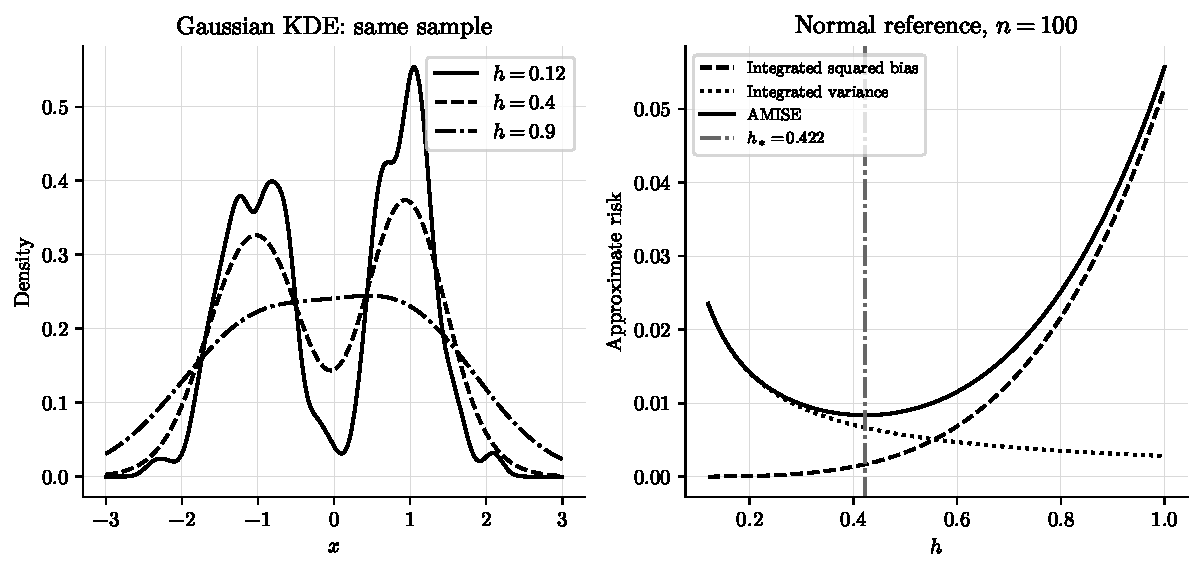
\includegraphics[width=.95\textwidth]{bandwidth_risk.pdf}
\caption{Trái: cùng mẫu, ba bandwidth KDE Gaussian. Phải: hai thành phần
AMISE và tổng của chúng trong mô hình chuẩn chuẩn tắc, $n=100$.
Các đường AMISE là xấp xỉ lý thuyết, không phải MISE thực nghiệm.}
\end{figure}
\intuition{Bandwidth nhỏ không miễn phí: giảm chệch nhưng tăng phương sai.
So sánh kernel cùng bậc thường thay đổi hằng số; thay bandwidth thay đổi
cả hai thành phần rủi ro theo các lũy thừa khác nhau.}
\source{\cite{slide2}, slide 25--26; \cite{wasserman}, trang in 133--135 (PDF 142--144)}

\section{Quy tắc tham chiếu chuẩn và Silverman}
\subsection{Dẫn ra hệ số 1.06}
Giả sử dùng kernel Gaussian và lấy mật độ chuẩn $N(\mu,\sigma^2)$ làm
tham chiếu. Với $z=(x-\mu)/\sigma$,
\[
f(x)=\frac1\sigma\varphi(z),\qquad
f''(x)=\frac{z^2-1}{\sigma^3}\varphi(z).
\]
Vì $dx=\sigma\,dz$,
\begin{align*}
R(f'')&=\frac1{2\pi\sigma^5}\int(z^2-1)^2e^{-z^2}\,dz\\
&=\frac1{2\pi\sigma^5}
\left(\frac{3\sqrt\pi}4-2\frac{\sqrt\pi}2+\sqrt\pi\right)
=\frac{3}{8\sqrt\pi\sigma^5}.
\end{align*}
Các tích phân được tính từ $\int e^{-z^2}=\sqrt\pi$ và tích phân từng
phần $\int z^{2k}e^{-z^2}=(2k-1)\int z^{2k-2}e^{-z^2}/2$.
Hạng biên $z^{2k-1}e^{-z^2}$ về 0 ở hai đầu.
Với Gaussian, $\mu_2(K)=1$, $R(K)=1/(2\sqrt\pi)$, nên
\[
h_*^5=\frac{1/(2\sqrt\pi)}{3/(8\sqrt\pi\sigma^5)n}
=\frac{4\sigma^5}{3n},\qquad
\boxed{h_{\rm NR}=(4/3)^{1/5}\sigma n^{-1/5}
\approx1.059224\sigma n^{-1/5}.}
\]
Thay $\sigma$ bằng độ lệch chuẩn mẫu $s$ cho $1.06s n^{-1/5}$.
Mô hình chuẩn là giả thiết dùng để tính bandwidth, không phải kết luận
rằng dữ liệu thật có phân phối chuẩn.

\subsection{Các phiên bản thực hành cần phân biệt}
Ở $N(\mu,\sigma^2)$, $\IQR=2\Phi^{-1}(0.75)\sigma\approx1.349\sigma$.
Đặt $a=\min\{s,\IQR/1.34\}$. Wasserman dùng $1.06a n^{-1/5}$
cho quy tắc tham chiếu chuẩn; quy tắc Silverman bền vững thường viết
$0.9a n^{-1/5}$. Hệ số $0.9$ không xuất phát từ cùng phép tối ưu chuẩn
vừa chứng minh.
Trong bài số của giáo trình, nếu không ghi khác, dùng
$s^2=(n-1)^{-1}\sum_i(X_i-\overline X)^2$ và hệ số chính xác
$(4/3)^{1/5}$, rồi mới làm tròn thành 1.06 khi cần minh họa.
Nếu tính IQR, dùng quantile thực nghiệm đã định nghĩa ở Chương 1;
các phần mềm nội suy có thể cho IQR khác ở mẫu nhỏ.
Nếu $s=0$, công thức cho bandwidth 0, không hợp lệ cho KDE:
phải có thông tin về độ phân giải hoặc chọn một bandwidth dương bên ngoài
quy tắc; không âm thầm chia cho 0.
\intuition{Quy tắc chuẩn nhanh vì thay đại lượng khó $R(f'')$ bằng công
thức của một mật độ tham chiếu. Mật độ nhiều đỉnh hoặc có đỉnh hẹp có thể
bị làm trơn quá mức; CV là một lựa chọn khác.}
\source{\cite{slide2}, slide 27; \cite{wasserman}, trang in 135 (PDF 144)}

\section{LOOCV cho KDE: công thức hữu hạn mẫu chính xác}
Giữ cùng $h$ khi bỏ quan sát:
\[
\widehat f_{(-i),h}(X_i)=\frac1{(n-1)h}
\sum_{j\ne i}K((X_i-X_j)/h).
\]
Với $n\geq2$, dùng
\[
\widehat J(h)=\int\fhat^2(x)\,dx
-\frac2n\sum_i\widehat f_{(-i),h}(X_i).
\]
Để tính tích phân đầu, khai triển bình phương thành tổng đôi. Trong cặp
$(i,j)$, đặt $u=(x-X_i)/h$, $dx=h\,du$:
\[
\int\frac1{h^2}K((x-X_i)/h)K((x-X_j)/h)\,dx
=\frac1h\int K(u)K(u+(X_i-X_j)/h)\,du.
\]
Đặt $C_K(v)=\int K(u)K(u+v)\,du$. Với kernel chẵn,
$C_K=K*K$ và ký hiệu $K^{(2)}$ thường được dùng.
Suy ra công thức chính xác
\[
\boxed{\widehat J(h)=\frac1{n^2h}\sum_{i,j}C_K((X_i-X_j)/h)
-\frac2{n(n-1)h}\sum_{i\ne j}K((X_i-X_j)/h).}
\]
Tổng đầu có đường chéo, tổng sau không có. Với Gaussian,
\[
C_K(v)=\frac1{2\sqrt\pi}e^{-v^2/4},
\]
là mật độ $N(0,2)$, có độ lệch chuẩn $\sqrt2$, không phải 2.
Với Uniform, $C_K(v)=(2-|v|)_+/4$, vì tích hai chiều cao bằng $1/4$
trên khoảng giao dài $(2-|v|)_+$.

\step{Tính không chệch của tiêu chuẩn.}
$X_i$ độc lập với mẫu bỏ $i$, nên
$\E\widehat f_{(-i),h}(X_i)=\int f_h(x)f(x)\,dx$.
Mặt khác $\E\fhat=f_h$ dù dùng $n$ hay $n-1$ quan sát.
Khai triển MISE cho
\[
\boxed{\E\widehat J(h)=\MISE_n(h)-R(f).}
\]
Điều kiện $f\in L_2$, $K\in L_1\cap L_2$ đảm bảo các hạng này hữu hạn.
Đẳng thức đúng cho $h$ cố định; chọn cực tiểu theo dữ liệu không làm
$\widehat J(\widehat h)$ thành ước lượng không chệch của rủi ro được chọn.

Trong thực hành, chọn một tập hữu hạn bandwidth dương và lấy điểm CV nhỏ
nhất; nếu bằng nhau, quy ước chọn bandwidth lớn hơn để ưu tiên làm trơn.
Một ứng viên nhỏ nhất ở mép lưới là tín hiệu cần kiểm tra phạm vi lưới.
Không có bảo đảm rằng CV hữu hạn mẫu luôn chọn tốt nhất; với dữ liệu
trùng lặp, bandwidth cực nhỏ có thể gây hành vi suy biến.
\intuition{LOO loại sự tự đóng góp $K(0)/(nh)$ của mỗi điểm. Tổng đôi
chính xác giúp tính CV mà không cần tích phân số cả một đường KDE.}
\source{\cite{wasserman}, trang in 135--136 (PDF 144--145), phương trình 6.33;
ở đây giữ mẫu số $n-1$ chính xác thay vì dùng dạng xấp xỉ 6.35}

\section{Nhân bậc cao}
Trong tài liệu này, kernel bậc $\ell$ nghĩa là
\[
\int K=1,\quad\mu_j(K)=0\ (1\leq j<\ell),\quad\mu_\ell(K)\ne0.
\]
Đây là một quy ước; Tsybakov dùng cách đặt tên khác cho số moment bị
triệt tiêu. Luôn kiểm tra các moment thực tế thay vì chỉ đọc chữ ``bậc''.
Với $f$ có đủ đạo hàm, moment tuyệt đối bậc $\ell$ hữu hạn và điều kiện
phần dư thích hợp,
\[
\Bias(\fhat(x))=
\frac{(-h)^\ell}{\ell!}\mu_\ell(K)f^{(\ell)}(x)+o(h^\ell).
\]
Tất cả hạng bậc thấp mất nhờ moment bằng 0.
Nếu khai triển đúng theo $L_2$, MISE có phần chính
$Ah^{2\ell}+R(K)/(nh)$, nên
\[
h_*\asymp n^{-1/(2\ell+1)},\qquad
\MISE=O(n^{-2\ell/(2\ell+1)}).
\]
Không thể dùng tốc độ này khi mật độ không có độ trơn tương ứng.

\begin{example}[Kernel Gaussian bậc bốn]
Đặt $K_4(u)=(3-u^2)\varphi(u)/2$.
Moment chuẩn tắc cho $\E Z^2=1$, $\E Z^4=3$, $\E Z^6=15$:
\[
\int K_4=(3-1)/2=1,\quad
\mu_2(K_4)=(3-3)/2=0,\quad
\mu_4(K_4)=(9-15)/2=-3.
\]
Moment lẻ bằng 0 do đối xứng. Vậy đây là kernel bậc bốn theo quy ước
trên, cho bias $-h^4f^{(4)}(x)/8+o(h^4)$ và tốc độ $n^{-8/9}$.
Nhưng $K_4(u)<0$ khi $|u|>\sqrt3$: KDE có thể âm.
\end{example}
Một kernel không âm, chuẩn hóa không thể có $\mu_2=0$ trừ một phân
phối tập trung tại 0, vốn không phải kernel mật độ thông thường:
$u^2K(u)\geq0$ mà tích phân bằng 0 thì $K=0$ hầu khắp nơi ngoài 0.
Do đó triệt tiêu moment bậc hai buộc kernel thông thường có phần âm.
\intuition{Nhân bậc cao dùng các vùng âm để bù chệch của vùng dương.
Đổi lại tốc độ nhanh hơn trên hàm rất trơn là mất tính không âm và
tăng yêu cầu về độ trơn của mật độ.}
\source{\cite{slide2}, slide 22; \cite{tsybakov}, Mục 1.2.2}

\section{Lớp Hölder và chặn rủi ro}
\subsection{Định nghĩa không suy biến ở bậc nguyên}
Với $\beta>0$, đặt $r=\lceil\beta\rceil-1$, $\eta=\beta-r\in(0,1]$.
Một hàm trong $\Sigma(\beta,L)$ có đạo hàm liên tục đến bậc $r$ và
\[
|f^{(r)}(x)-f^{(r)}(y)|\leq L|x-y|^\eta.
\]
Đồng thời yêu cầu $f\geq0$, $\int f=1$ khi xét lớp mật độ;
dùng thêm chặn $\norm f_\infty\leq M$ khi chứng minh chặn phương sai.
Với $r=0$ đây là điều kiện trực tiếp trên $f$; với $\beta=2$, $f'$ là
Lipschitz. Không viết $|f(x)-f(y)|\leq L|x-y|^\beta$ cho mọi
$\beta>1$ trên một khoảng: điều kiện ấy buộc $f$ hằng.

\subsection{Chặn bias bằng Taylor có phần dư Hölder}
Taylor đến bậc $r$ cho
\[
f(x+t)=\sum_{j=0}^r\frac{f^{(j)}(x)}{j!}t^j+\mathcal R_\beta,
\qquad |\mathcal R_\beta|\leq\frac{L}{r!}|t|^\beta.
\]
Với $r=0$ đây chính là định nghĩa. Với $r\geq1$, Taylor dạng tích phân
đến bậc $r-1$, rồi trừ và cộng $f^{(r)}(x)$ trong tích phân:
\[
\mathcal R_\beta=
\frac{t^r}{(r-1)!}\int_0^1(1-s)^{r-1}
[f^{(r)}(x+st)-f^{(r)}(x)]\,ds.
\]
Trị tuyệt đối bị chặn bởi $L|t|^{r+\eta}/(r-1)!$ nhân
$\int_0^1(1-s)^{r-1}s^\eta ds\leq1/r$; đó là chặn đã nêu.
Nếu kernel triệt tiêu moment $1,\ldots,r$ và
$M_\beta(K)=\int|u|^\beta|K(u)|\,du<\infty$, thì
\begin{align*}
\Bias(\fhat(x))&=\int K(u)\mathcal R_\beta(x,-hu)\,du,\\
\boxed{|\Bias(\fhat(x))|}&\boxed{\leq (L/r!)M_\beta(K)h^\beta.}
\end{align*}
Tính đối xứng chỉ tự triệt tiêu moment lẻ, không triệt tiêu mọi moment.

\subsection{Chặn variance và MSE}
Không cần Taylor để có chặn phương sai:
\[
\Var\fhat(x)\leq\frac1n\E Z_1(x)^2
=\frac1{nh}\int K^2(u)f(x-hu)\,du
\leq\boxed{\frac{MR(K)}{nh}}.
\]
Đặt $C_b=(L/r!)M_\beta(K)$, ta có
\[
\sup_f\MSE_f(\fhat(x))\leq C_b^2h^{2\beta}+\frac{MR(K)}{nh}.
\]
Chọn $h\asymp n^{-1/(2\beta+1)}$ cho chặn
$O(n^{-2\beta/(2\beta+1)})$. Đây là chặn đều \emph{tại điểm}; không
tích phân hằng số trên toàn $\R$ để suy ra MISE hữu hạn.
Để có MISE cùng bậc, dùng điều kiện độ trơn theo chuẩn $L_2$ như lớp
Sobolev, hoặc miền compact với xử lý biên và chặn bias đồng đều.
Phương sai tích phân luôn bị chặn bởi $R(K)/(nh)$.
\source{\cite{tsybakov}, Mệnh đề 1.1--1.2 và Định lý 1.1,
trang in 4--9 (PDF 15--20); Mệnh đề 1.4, trang in 12 (PDF 23)}

\subsection{Minimax: vì sao đây là tốc độ tốt nhất?}
Với lớp mật độ Hölder có chặn nêu trên và $x_0$ ở miền nội thích hợp,
đặt
\[
\mathcal R_n^*(x_0)=\inf_{T_n}\sup_{f\in\mathcal F}
\E_f[T_n-f(x_0)]^2.
\]
Infimum chạy trên mọi estimator đo được từ mẫu. Kết quả lower bound
cho lớp đủ phong phú là
\[
\mathcal R_n^*(x_0)\geq c n^{-2\beta/(2\beta+1)},
\]
với $c>0$ phụ thuộc lớp, không phụ thuộc $n$. Kết hợp chặn trên vừa chứng
minh cho tốc độ minimax. Chặn trên của riêng KDE không tự chứng minh
lower bound cho mọi estimator.

\step{Phác thảo lower bound tại điểm.}
Chọn mật độ nền $f_0$ dương quanh $x_0$, thêm một nhiễu
$\delta a^\beta\psi((x-x_0)/a)$ có $\int\psi=0$, $\psi(0)\ne0$,
compact và đủ trơn. Với $\delta$ nhỏ, mật độ mới $f_1$ vẫn không âm,
chuẩn hóa và ở cùng lớp. Hai giá trị tại $x_0$ cách nhau bậc $a^\beta$.
\[
\int\frac{(f_1-f_0)^2}{f_0}\,dx=O(a^{2\beta+1}),
\quad
\operatorname{KL}(P_1^n,P_0^n)=O(na^{2\beta+1}).
\]
Chọn $a\asymp n^{-1/(2\beta+1)}$ để hai luật mẫu khó phân biệt.
Lower bound kiểm định hai giả thuyết (Le Cam) buộc sai số bình phương
ít nhất có bậc $a^{2\beta}$. Đây là phác thảo, các bổ đề kiểm định được
viện dẫn từ \cite{tsybakov}, Chương 2.
Với rủi ro tích phân, đặt nhiều nhiễu trên các ô rời nhau và dùng
Assouad/Fano; Wasserman Định lý 6.31 cho lower bound MISE trên lớp
$R(f^{(m)})\leq c^2$, đạt $n^{-2m/(2m+1)}$.
\intuition{Độ trơn cho phép mượn thông tin ở lân cận. Lower bound nói
rằng dù chọn thuật toán nào, một lớp có nhiều nhiễu nhỏ khó phân biệt
vẫn đặt ra giới hạn thông tin. Minimax là kết luận theo lớp và loại mất mát.}

\section{Chệch biên và cách xử lý}
Giả sử miền giá đỡ là $[0,\infty)$, $f(0+)>0$, kernel chẵn. Tại 0,
\[
\E\fhat(0)=\int_0^\infty\frac1hK(-t/h)f(t)\,dt
=\int_0^\infty K(u)f(hu)\,du.
\]
Nếu $f$ liên tục phải và điều kiện chi phối thỏa,
giới hạn bằng $f(0+)\int_0^\infty K=f(0+)/2$. Vì vậy
\[
\boxed{\Bias(\fhat(0))\to-f(0+)/2.}
\]
Chệch ngay tại biên có thể là $O(1)$, không phải $O(h)$.
Vùng biên rộng $O(h)$ với chệch không tiêu biến có thể làm squared bias
tích phân bậc $O(h)$ và phá tốc độ AMISE nội miền.

\subsection{Phản xạ}
Trên nửa trục, định nghĩa
\[
\widehat f_R(x)=\frac1{nh}\sum_i
\{K((x-X_i)/h)+K((x+X_i)/h)\},\quad x\geq0.
\]
Với kernel chẵn, tổng diện tích của hai bản kernel trên $[0,\infty)$
bằng 1 cho mỗi quan sát: phần bị cắt của bản tâm $X_i$ được bản tâm
$-X_i$ bù lại. Vì vậy estimator không âm và tích phân 1 trên nửa trục.
Tại 0,
\begin{align*}
\E\widehat f_R(0)
&=2\int_0^\infty K(u)f(hu)\,du\\
&=f(0+)+2hf'(0+)\int_0^\infty uK(u)\,du+O(h^2).
\end{align*}
Phản xạ bỏ chệch hằng số, nhưng nếu $f'(0+)\ne0$, bias vẫn $O(h)$.
Nếu $f'(0+)=0$ và đủ trơn, có thể đạt $O(h^2)$.
Với $f(x)=e^{-x}\1_{x\geq0}$ và Uniform,
$\E\fhat(0)=(1-e^{-h})/(2h)$,
$\E\widehat f_R(0)=(1-e^{-h})/h=1-h/2+O(h^2)$.

\subsection{Boundary kernel}
Ở biên 0, có thể dùng trọng số tương đương $L$ trên $[0,1]$ thỏa
$\int_0^1L=1$, $\int_0^1uL(u)du=0$. Ví dụ $L(u)=4-6u$ trên
$[0,1]$. Khi đó estimator
$(nh)^{-1}\sum_i L(X_i/h)\1_{\{0\leq X_i\leq h\}}$
có kỳ vọng $\int_0^1L(u)f(hu)du=f(0)+O(h^2)$.
Moment bậc một triệt tiêu cả khi cửa sổ chỉ một phía.
Nhưng $L$ có phần âm; estimator không tự động là mật độ không âm,
và đây là công thức \emph{tại biên}, không phải kernel chung cho toàn miền.
Chỉ chuẩn hóa lại kernel bị cắt mà không triệt tiêu moment bậc một
thường chỉ cải thiện bias về $O(h)$.

\begin{figure}[htbp]
\centering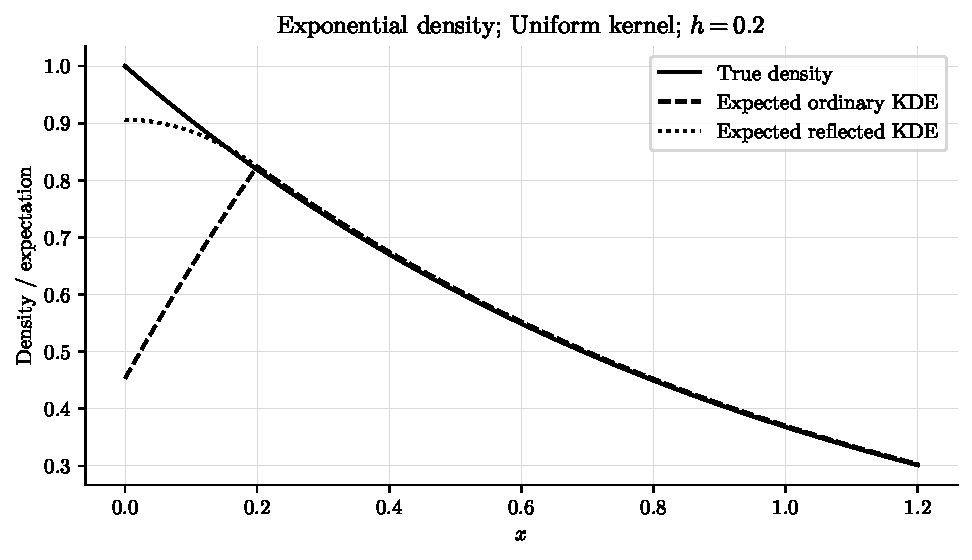
\includegraphics[width=.9\textwidth]{boundary.pdf}
\caption{Mật độ mũ và kỳ vọng KDE Uniform tại $h=0.2$.
Reflection sửa phần thiếu khối lượng nhưng vẫn còn chệch bậc nhất tại 0.
Đường vẽ là kỳ vọng tính giải tích, không phải KDE của một mẫu.}
\end{figure}
\intuition{Kernel đối xứng chỉ triệt tiêu moment lẻ khi có dữ liệu ở cả
hai phía. Ở biên, một phía không tồn tại nên phép triệt tiêu mất hiệu lực.}

\section{Suy luận thống kê cho mật độ: kiểm soát chệch}
Ở điểm nội với $f(x)>0$, kernel và mật độ thỏa điều kiện CLT cho mảng
tam giác, $h\to0$, $nh\to\infty$,
\[
\sqrt{nh}[\fhat(x)-\E\fhat(x)]\Rightarrow N(0,f(x)R(K)).
\]
CLT này canh tâm ở $f_h(x)=\E\fhat(x)$, không tự ở $f(x)$.
Nếu $h\asymp n^{-1/5}$, bias $h^2$ và độ lệch chuẩn $(nh)^{-1/2}$
cùng bậc. Muốn bỏ bias để suy luận cho $f(x)$, một điều kiện đủ là
\[
\sqrt{nh}\,h^2\to0\quad\Longleftrightarrow\quad nh^5\to0,
\]
đồng thời $nh\to\infty$; đây là undersmoothing.
Khi các điều kiện này thỏa, khoảng tại điểm xấp xỉ là
$\fhat(x)\pm z_{1-\alpha/2}\sqrt{R(K)\fhat(x)/(nh)}$ với kernel
mật độ không âm. Một băng đồng thời cần thêm kiểm soát supremum của
quá trình ngẫu nhiên, không chỉ lấy cùng hệ số chuẩn ở mọi $x$.
\intuition{Bandwidth tối ưu để ước lượng theo MSE chưa chắc phù hợp để
lập khoảng tin cậy bỏ qua bias. Chương 5 tiếp tục vấn đề này với Root--Unroot.}
\source{\cite{slide2}, slide 28; \cite{wasserman}, Chương 5, Mục 5.7 và Chương 6}
